%%____________________________________________________________________________||
\section{Aggregate signal regions}
\label{sec:aggregate-signal-regions}

Inclusive searches for new physics typically use fine categorisation to allow
sensitivity to a wide range of models. However, this can make the use
of the search for re-interpretation impractical. This section describes how this categorisation
may be simplified without breaking the correlation between the bins through defining aggregate regions
\footnote{In this section a binned analysis is considered, however, the extension to searches using continous functions for signal
and background modelling is trivial.}. The aggregate regions may be defined with 
the original likelihood or, approximately, with the predictions and covariance matrix. 

A generic binned likelihood is defined in Equation~\ref{eq:generic-binned-likelihood}. 

\begin{equation}
 \mathcal{L}(\mu, \boldsymbol{\theta}) = 
 \prod_i(\mathrm{data_i}|\mu\cdot s_i(\boldsymbol{\theta}) + b_i(\boldsymbol{\theta})) \cdot p(\tilde{\boldsymbol{\theta}}|\boldsymbol{\theta})
\label{eq:generic-binned-likelihood}
\end{equation}

where the product is over all bins in the search. To define aggregate regions the 
predictions in the bins being aggregated is summed while maintaining all
information on the nuisance parameters. The aggregate likelihood is therefore defined
in Equation ~\ref{eq:agg-generic-binned-likelihood}.
\begin{equation}
 \mathcal{L}(\mu, \boldsymbol{\theta}) = 
 \prod_I(\sum_i\mathrm{data_i}|\sum_i(\mu\cdot s_i(\boldsymbol{\theta}) + b_i(\boldsymbol{\theta}))) \cdot p(\tilde{\boldsymbol{\theta}}|\boldsymbol{\theta})
\label{eq:agg-generic-binned-likelihood}
\end{equation}

where the sum is over all bins used to define each aggregate region, $I$.
The aggregate regions may then be used to derive the predictions and covariance that may be
used for the simplified likelihood discussed in 
Section~\ref{sec:simplified-likelihood}. Note that the probability density for the nuisance
parameters is unchanged.

An alternative derivaration of the predictions and covariance of aggregate region 
required for the simplified likelihood definition in Equation~\ref{eq:full-likelihood} can
be made using the predictions and covariance of the nominal signal regions discussed in 
Section~\ref{sec:simplified-likelihood}.
These can be merged using Equation~\ref{eq:agg-cov}. For the covariance of the aggregate
region to be accurate relies on the same conditions on the nuisances outlined 
in Section~\ref{sec:simplified-likelihood}. 

\begin{align}
b_{I} = \sum_i b_{i} && V_{IJ}=\sum_{ij}V_{ij}
\label{eq:agg-cov}
\end{align}

where the sum is over all regions being aggregated. The aggregate predictions
and covariance can then be used to define the simplified likelihood.

\subsection{Example of the use of aggregate regions}
\label{sec:agg-toy}

The same toy model is considered as in Section~\ref{sec:sl-toy}. From Figure~\ref{fig:toy-example}
it is clear that only search regions 7 and 8 exhibit large contributions from the signal
model. One may therefore expect that regions 1-6 can be neglected when setting limits. 
However, as these bins are correlated, if regions 1-6 are not considered information 
on the nuisances in the regions with large signal contributions is lost. 
Alternatively, the regions 1-6 may be aggregated using the covariance matrix shown in 
Figure~\ref{fig:covariance} using Equation~\ref{eq:agg-cov}. The resulting covariance
between the aggregate regions is shown in Figure~\ref{fig:agg-covariance}.

\begin{figure}[hbt]
  \begin{center} 
   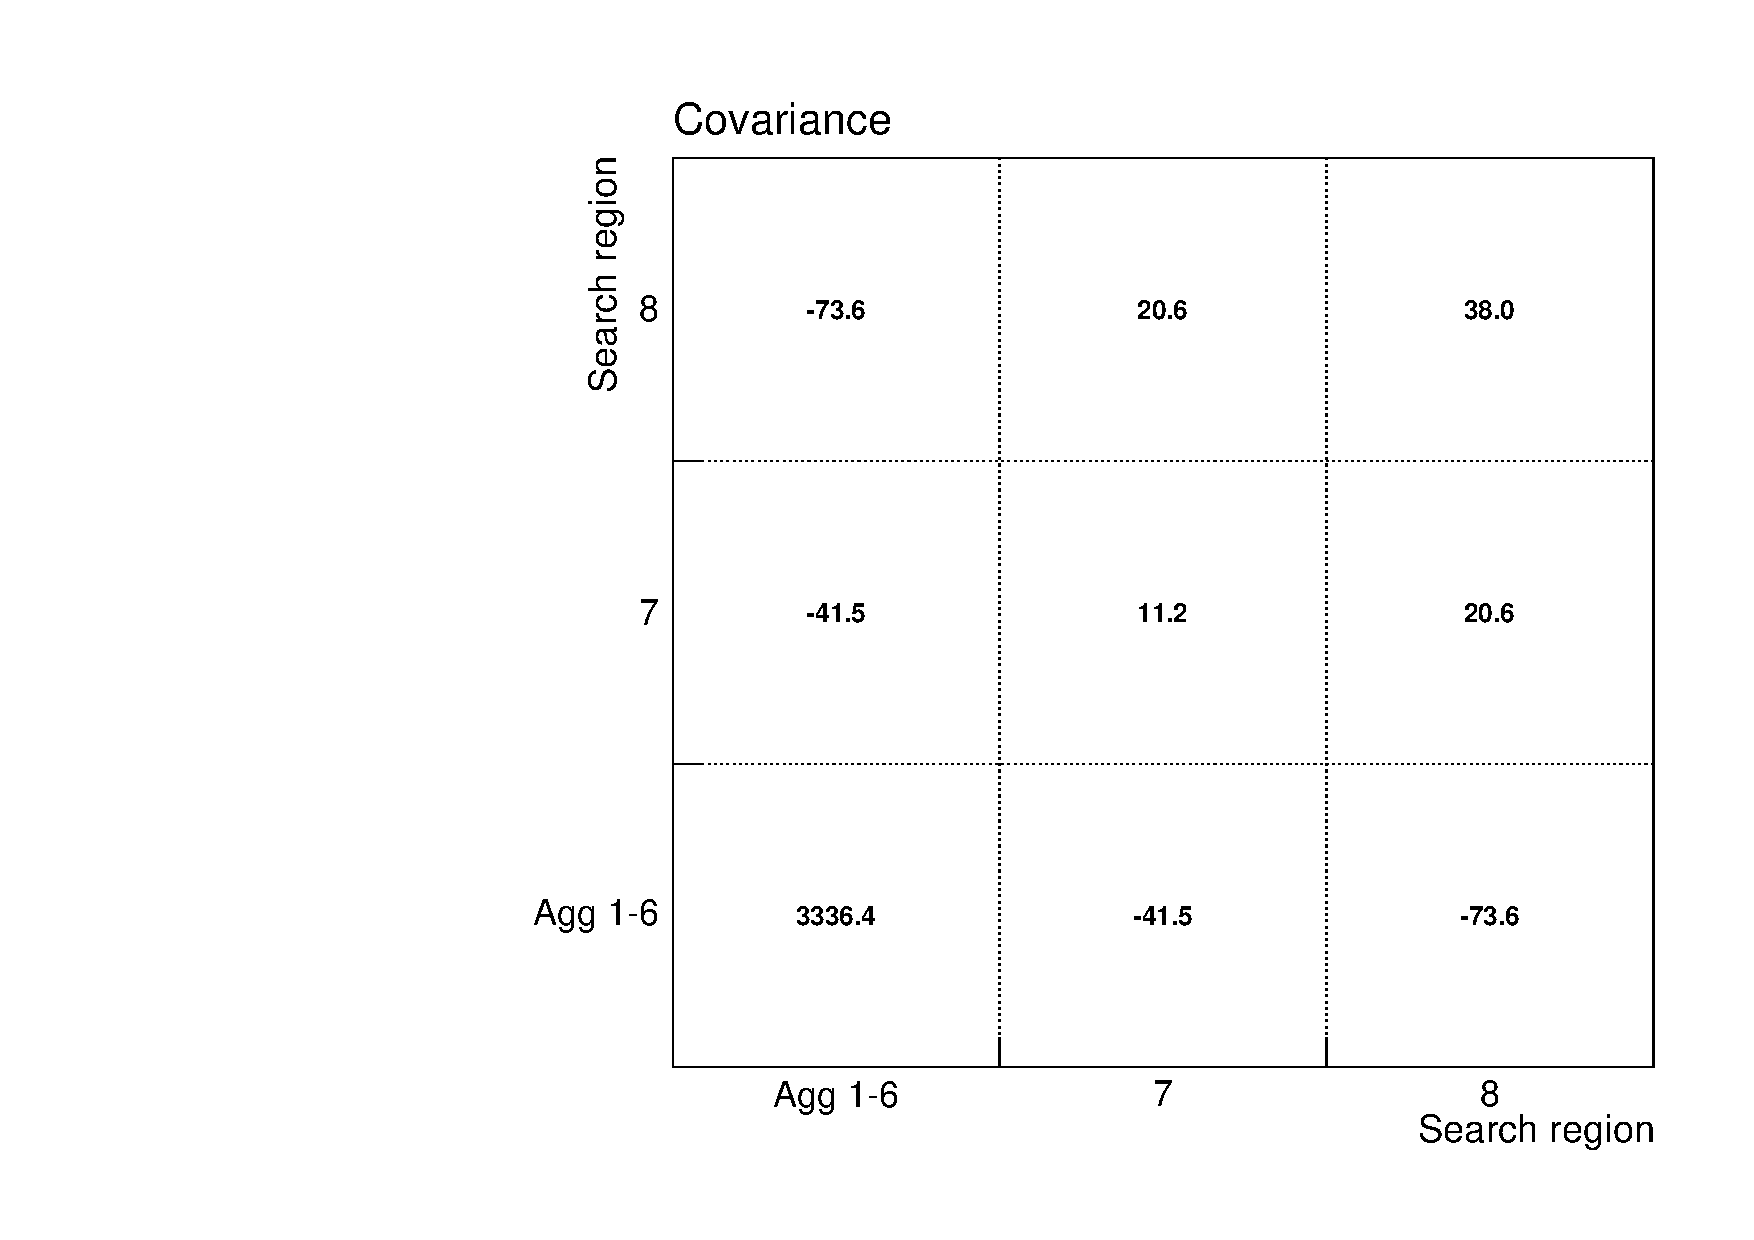
\includegraphics[width=1.5\cmsFigWidth]{figures/agg_htsearch_covariance.pdf}
   \caption{Covariance between the total rate of background contributions expected in each of the aggregated search regions}
   \label{fig:agg-covariance} 
  \end{center}
\end{figure}

Figure~\ref{fig:agg-likelihoodscan} shows the value of $q(\mu)$ as a function of $\mu$. The values when $q(\mu)$ 
is defined using the likelihood of Equation~\ref{eq:full-likelihood} for the nominal signal region, the aggregated signal
regions described above, and considering search regions 7 and 8 only are shown. The aggregated regions show
good agreement compared to the nominal while neglecting the regions 1-6 is shown to introduce a considerable
bias in the estimate of $\hat{\mu}$. In addition, the width of the likelihood curve when neglecting these regions is considerably
larger, implying a larger uncertainty estimate on $\mu$. This can be expected from the loss of information on
the systematic uncertainties when search regions 1-6 are neglected. Generically, the impact of removing regions
will be dependant on the size of the systematic uncertainties and correlations between the regions used and those
dropped.

\begin{figure}[hbt]
  \begin{center} 
   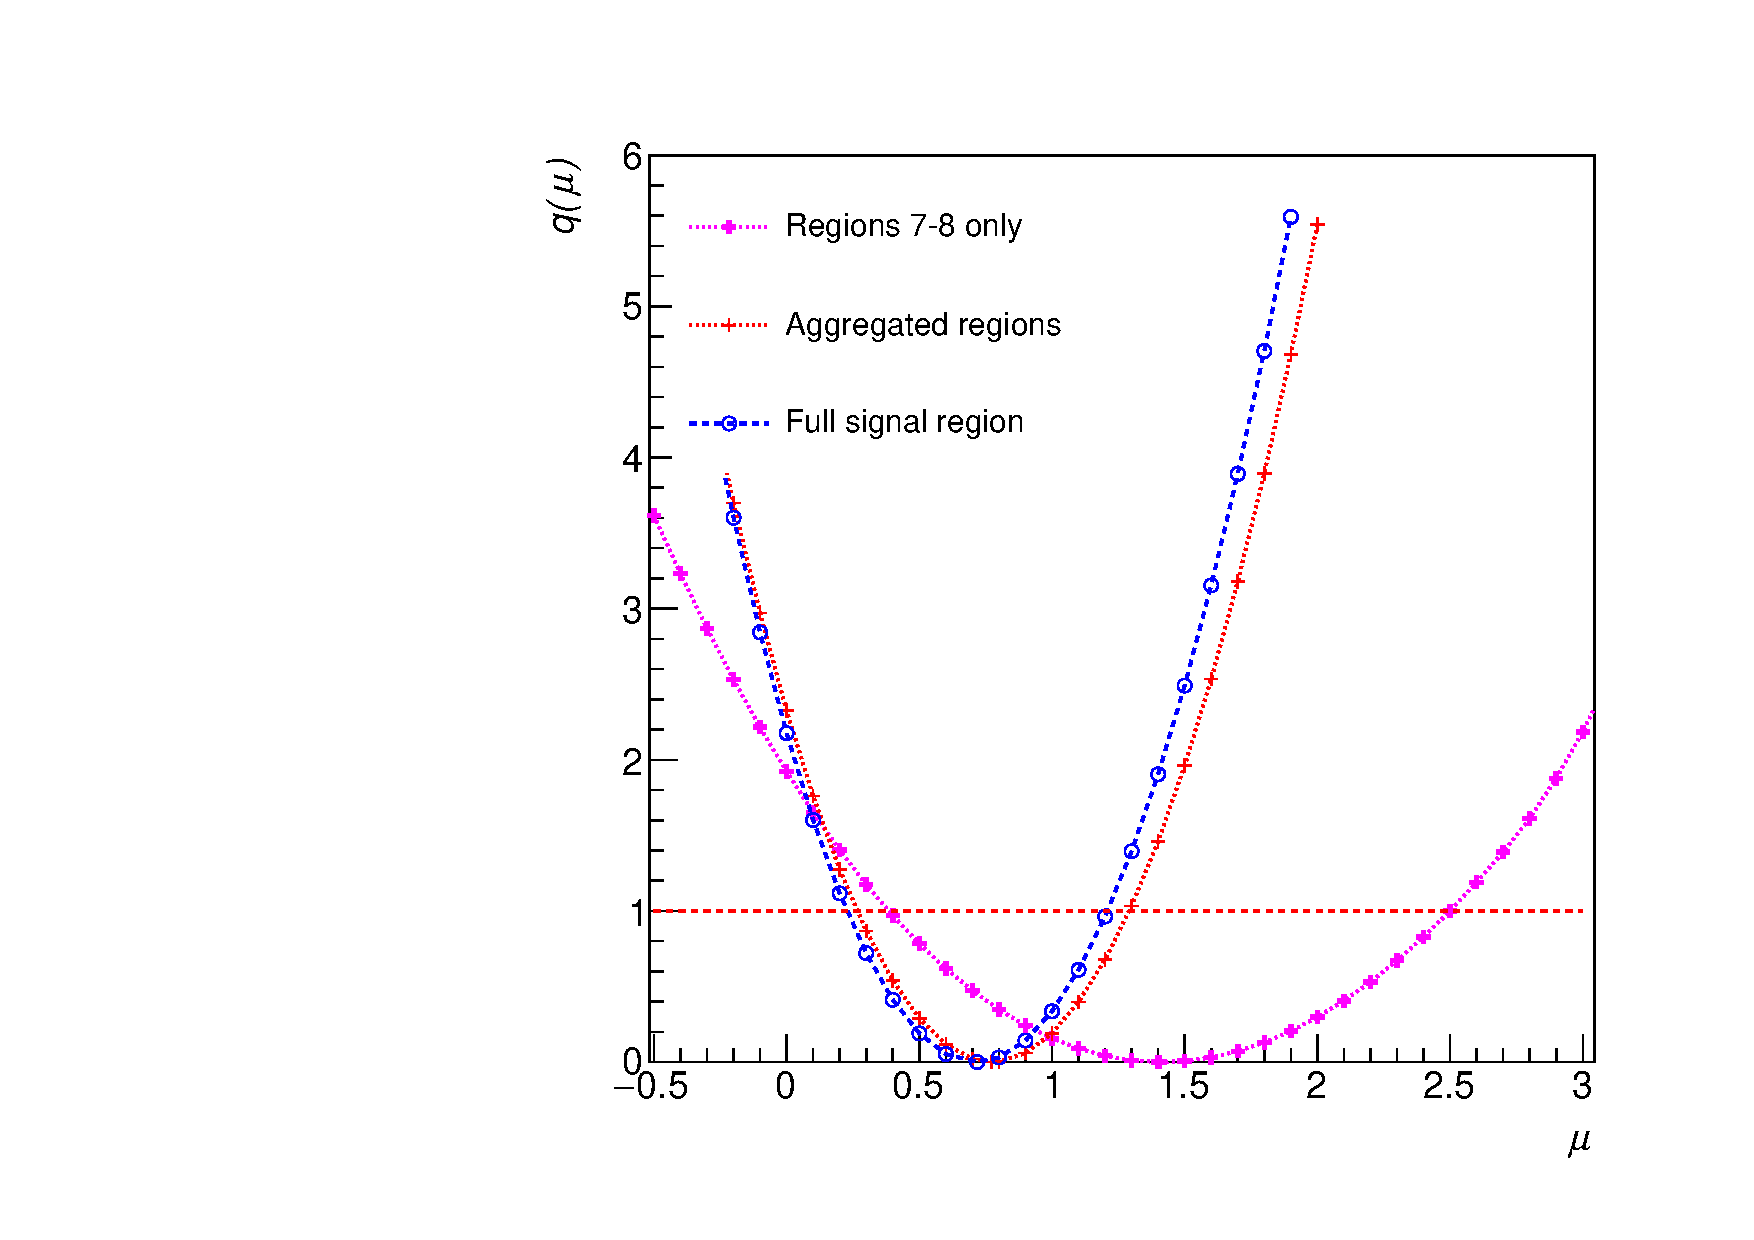
\includegraphics[width=1.5\cmsFigWidth]{figures/r_agg.pdf}
   \caption{The value of $q(\mu)$ defined using the simplified likelihood using the full signal region (open blue points), the aggregated signal region (thin red crosses),
   and regions 7-8 only (open magenta crosses).}
   \label{fig:agg-likelihoodscan} 
  \end{center}
\end{figure}
